\chapter{実験}
\label{implementation}


\section{実験環境}
理想のポーズとなる関節角度を指定した3Dモデルを2つ作成する。ポーズはダブルバイセップス 図\ref{fig:pose1}、クラシックポーズ 図\ref{fig:pose2}である。\\ \indent	
被験者を2つの群に分ける。グループ1はpose1を本システムで練習し、pose2を鏡を使って練習する。グループ2はpose1を鏡を使って練習し、pose2を本システムを使って練習する。
\\ \indent
システムを使用する練習、鏡を使用する練習それぞれで、30秒ポージング、30秒休みを1セットとし、計10セット行った。
\begin{figure}[htbp]
  \begin{center}
      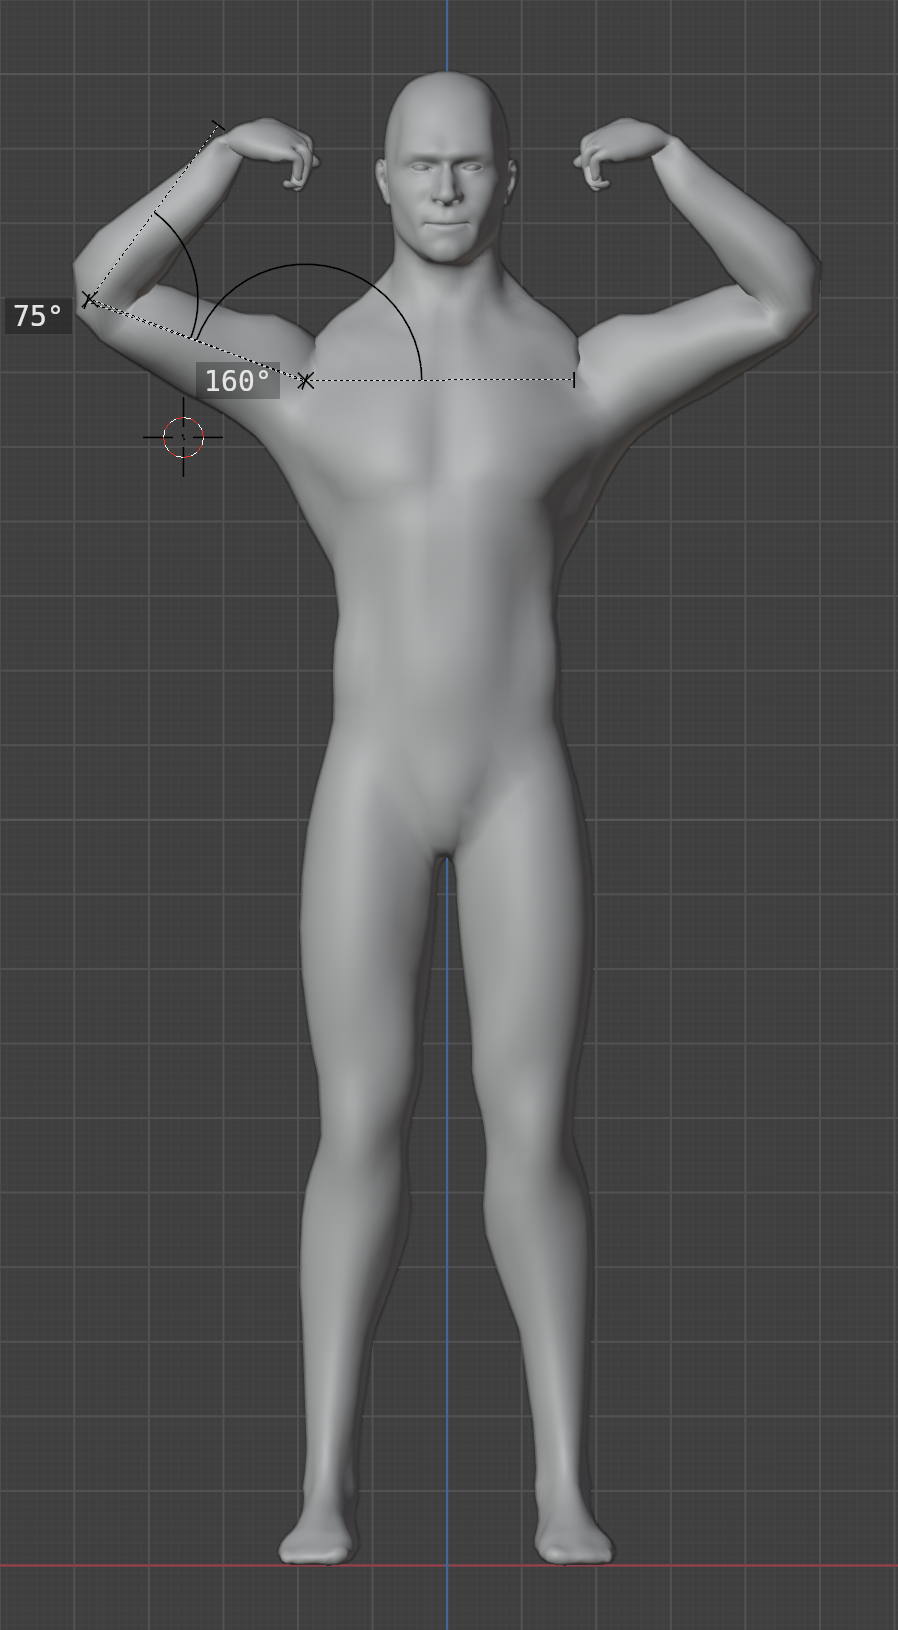
\includegraphics[width=7cm]{figures/pose1.png}
      \caption{ダブルバイセップス(pose1)}
      \label{fig:pose1}
  \end{center}
\end{figure}
\begin{figure}[htbp]
  \begin{center}
      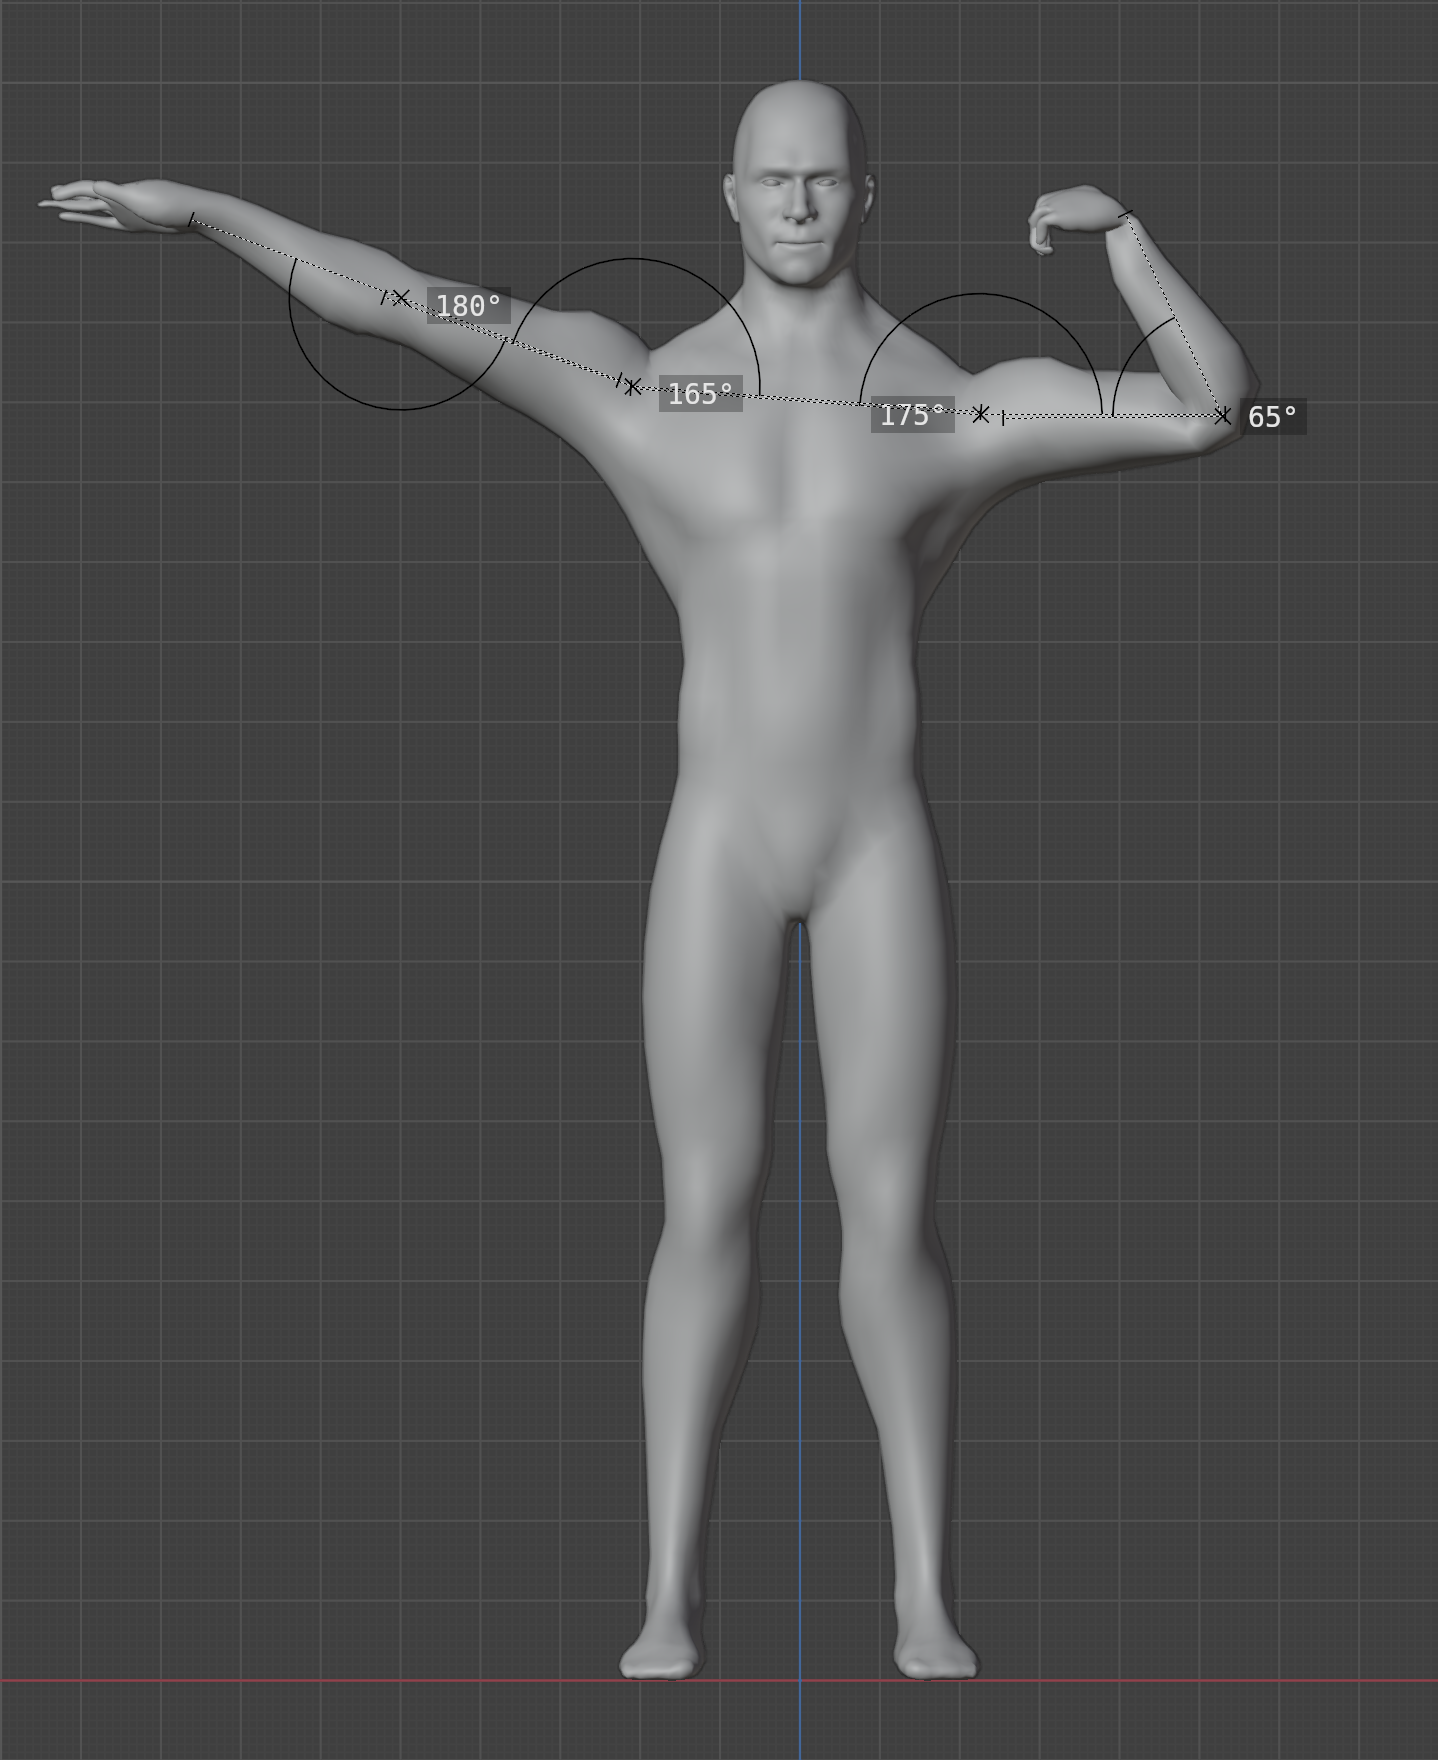
\includegraphics[width=10cm]{figures/pose2.png}
      \caption{クラシックポーズ(pose2)}
      \label{fig:pose2}
  \end{center}
\end{figure}
